
\subsubsection{Resistenze interne strumenti}
%    
    Chiamiamo $R_i$ la resistenza da misurare e $R_V$ la resistenza interna del voltmetro e $R_A$ la resistenza interna dell'amperometro.\\    
%  
    Le resistenze che abbiamo utilizzato sono le seguenti (errore letto da ultima cifra dello strumento di misura):
    %   Tabella dati resistenze
    \begin{table}[H]
        \centering
        \begin{tabular}{|l r|}
            \hline
            $R_1$ & $ 10.1 \pm 0.1\Omega$      \\
            $R_2$ & $ 677 \pm 1\Omega$         \\
            $R_3$ & $ 15970 \pm 10\Omega$      \\
            $R_4$ & $ 981000 \pm 1000\Omega$   \\ 
            $R_5$ & $ 149000 \pm 100\Omega$    \\ 
            \hline
        \end{tabular}
        %\caption{Caption}
        %\label{tab:my_label}
    \end{table}
    
    Schema dei due circuiti:
     % Schema circuiti
    \begin{figure}[H]
    \centering
    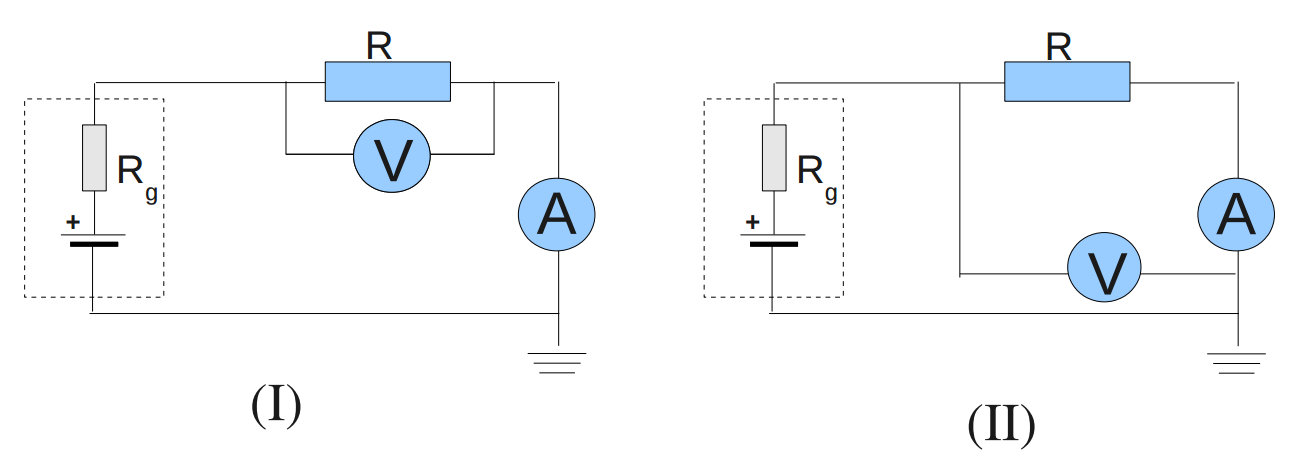
\includegraphics[scale=.25]{Grafici/C1_P1.png}
    \end{figure} 
    
    
    Formule utilizzate:
    $$ \Delta V = R_{eq} I \Rightarrow R_{eq}=\frac{\Delta V}{I}$$

    %spiegazione Rv
    Circuito 1: misura di $R_V$
    $$ \frac{1}{R_{eq}} = \frac{1}{R} + \frac{1}{R_V} \Rightarrow R_V = \frac{RR_{eq}}{R-R_{eq}} = \frac{R \Delta V}{IR - \Delta V} $$
    
    
    %spiegazione Ra
    Circuito 2: misura di $R_A$
    $$ R_{eq} = R + R_A \Rightarrow R_A = R_{eq} - R = \frac{\Delta V}{I} - R$$
    
    
    %   resistenza bassa
    %Abbiamo riscontrato che se $R$ è troppo bassa rispetto a $R_V$, le misure effettuate risultano alterate. Abbiamo attribuito questo effetto alla eccessiva differenza tra le due resistenze, che fa sì che la corrente passante attraverso $R_V$ non sia sufficiente per una misura corretta.  
   % Riportiamo in seguito i dati relativi a ciò.
%
    %   tabella schifo
    %\begin{table}[H]
\caption{Misure di $R_V$ usando resistenze basse}
\begin{tabular}{|c|c|c|c|c|}
\hline
Tensione V (V) & Corrente I (A) & Resistenza R ($\Omega$) & \textbf{Rv ($\Omega$)} & $fem$ (V) \\
\hline
0.561 & 5.75E-02 & 10.1 & 2.87E+02 & 0.90 \\ 
0.937 & 9.57E-02 & 10.1 & 3.20E+02 & 1.50 \\ 
1.657 & 1.69E-01 & 10.1 & 3.35E+02 & 2.00 \\ 
0.997 & 1.48E-03 & 677 & 4.29E+05 & 1.00 \\ 
2.982 & 4.41E-03 & 677 & 4.10E+05 & 3.00 \\
5.45 & 8.08E-03 & 677 & 2.20E+05 & 5.50 \\ \hline
\end{tabular}
\label{}
\end{table}
% 
%
    Dati sperimentali:
    %Tabella dati Rv%
    \begin{table}[H]
    \centering
    \caption{Misure di Resistenza Voltmetro}
    \begin{tabular}{|c|c|c|c|}
    \hline
        Tensione V(V) & Corrente I(A) & Resistenza R (k$\Omega$) & Resistenza $R_V$ ($\Omega$) \\
        $\pm 0.01\%$ & $\pm 3.92 \%$ & $\pm 0.27 \%$ & $\pm 4.47 \%$\\
        \hline
        5.504   & $3.45 \cdot10^{-1}$  & 15.97  & $1.56 \cdot10^4$ \\
        4.012   & $2.52 \cdot10^{-1}$  & 15.97  & $5.15 \cdot10^3$ \\
        6.507   & $4.08 \cdot10^{-1}$  & 15.97  & $1.19 \cdot10^4$ \\
        13.04   & $1.50 \cdot10^{-2}$  & 981.0  & $7.64 \cdot10^3$ \\
        7.510   & $8.00 \cdot10^{-3}$  & 981.0  & $2.18 \cdot10^4$ \\
        10.02   & $1.10 \cdot10^{-2}$  & 981.0  & $1.27 \cdot10^4$ \\
        5.012   & $3.40 \cdot10^{-2}$  & 149.0  & $1.38 \cdot10^4$ \\
        8.010   & $5.50 \cdot10^{-2}$  & 149.0  & $6.45 \cdot10^3$ \\
        11.02   & $7.50 \cdot10^{-2}$  & 149.0  & $1.06 \cdot10^4$ \\
        \hline
    \end{tabular}
    \label{}
\end{table} 
    %Tabella dati Ra
    \begin{table}[H]
    \centering
    \caption{Misure di Resistenza Amperometro}
    \begin{tabular}{|c|c|c|c|}
    \hline
        Tensione V(V) & Corrente I(A) & Resistenza R ($\Omega$) & Resistenza $R_A$ ($\Omega$) \\
        $\pm 0.03\%$ & $\pm 0.09 \%$ & $\pm 0.04 \%$ & $\pm 0.20 \%$\\
        \hline
            4.001 & 1.455 $\cdot 10^{-2}$ & 267.6 & 7.38 \\ 
            7.010 & 2.580 $\cdot 10^{-2}$ & 267.6 & 4.11 \\ 
            1.506 & 5.509 $\cdot 10^{-3}$ & 267.6 & 5.77 \\ 
            2.506 & 9.170 $\cdot 10^{-3}$ & 267.6 & 5.68 \\ 
            8.510 & 3.140 $\cdot 10^{-2}$ & 267.6 & 3.42 \\ \hline
    \end{tabular}
    \label{}
\end{table}

    
    
    Per $R_V$ e $R_A$, abbiamo stimato l'errore relativo percentuale dalla somma degli errori relativi di $V$ $R$ e $I$, trovando:
        $$ R_V = 1.17\cdot10^4 \; k\Omega \pm 4.47\%$$
        $$ R_A = 5.27 \Omega \pm 0.02 \% $$
% 
%
%
%
%
\subsubsection{Verifica legge di Ohm}
%
% 
%   
\textbf{Resistore 1}\\
%
    % Dati R1
    \begin{table}[H]
    \centering
    \begin{tabular}{|c|c||c|c|}
    \hline
        Tensione V 	&	Corrente I & Tensione V   &   Corrente I 	\\
        V	&	mA      & V &   mA	\\
        $\pm 0.001 (0.04\%)$	&	$\pm 0.01 $ & $\pm 0.001 (0.04\%)$   &   $\pm 0.01 $	\\ \hline
        0.503	&	0.74	&  5.459   &   8.09    \\
        0.996	&	1.47	&  5.949   &   8.81    \\
        1.497	&	2.21	&  6.446   &   9.56    \\
        1.992	&	2.95	&  6.950   &   10.30   \\
        2.488	&	3.68	&  7.440   &   11.03   \\
        2.982	&	4.41	&  7.940   &   11.78   \\
        3.473	&	5.14	&  8.430   &   12.52   \\
        3.972	&	5.88	&  8.930   &   13.27   \\
        4.471	&	6.62	&  9.430   &   14.00   \\
        4.964	&	7.35	&  9.920   &   14.75   \\ \hline
    \end{tabular}
    \caption{Dati per R1}
    \label{tab:R1_ohm}
\end{table}
%
    % Grafico R1
    \begin{figure}[H]
    \centering
    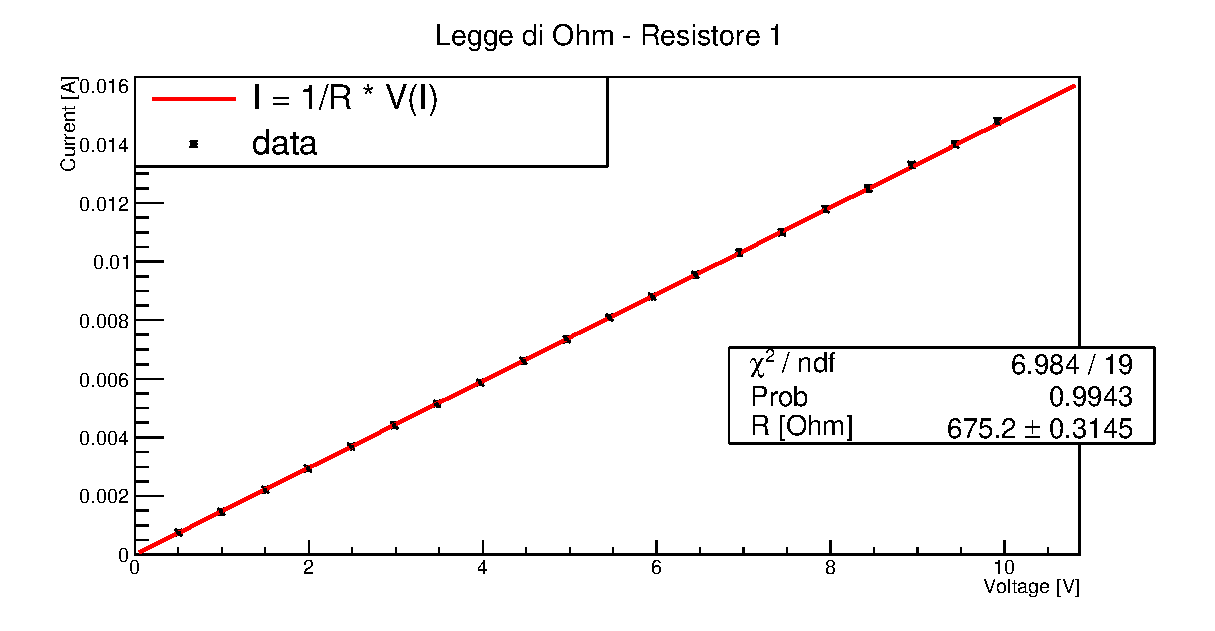
\includegraphics[scale=.8]{Grafici/C1_P1_ohmR1.eps}
    %\caption{Verifica legge di Ohm per resistore R1}
    \label{fig:C1_P1_OhmR1}
    \end{figure} 
%
    %   Resistore R1
    \begin{center}
   % \centering
    Valore misurato: $R_1 = 677 \pm 1  \Omega$  \\
    Valore ottenuto dal Fit: $R_1 = 675.2 \pm 0.3 \Omega$ \\
    \end{center}
%
    Il risultato è accurato anche se l'errore associato è probabilmente troppo basso.\\\\
%
% 
%
%
%
\textbf{Resistore 2}\\
%
    % Dati R2
    \begin{table}[H]
    \centering
    \begin{tabular}{|c|c||c|c|}
    \hline
        Tensione V 	&	Corrente I & Tensione V   &   Corrente I 	\\
        V	&	mA      & V &   mA	\\
        $\pm 0.001 (0.04\%)$	&	$\pm 0.01 $ & $\pm 0.001 (0.04\%)$   &   $\pm 0.01 $	\\ \hline
        0.249   &   0.94    &   2.699   &   10.15   \\
        0.493   &   1.89    &   2.940   &   11.05   \\
        0.744   &   2.80    &   3.184   &   11.98   \\
        0.983   &   3.96    &   3.427   &   12.89   \\
        1.233   &   4.63    &   3.674   &   13.83   \\
        1.477   &   5.55    &   3.914   &   14.73   \\
        1.722   &   6.47    &   4.163   &   15.68   \\
        1.959   &   7.36    &   4.403   &   16.59   \\
        2.212   &   8.31    &   4.652   &   17.52   \\
        2.448   &   9.21    &   4.892   &   18.44   \\ \hline
    \end{tabular}
    \caption{Dati per R2}
    \label{tab:R2_ohm}
\end{table}




       
        
        
%
    %   Grafico R2
    \begin{figure}[H]
    \centering
    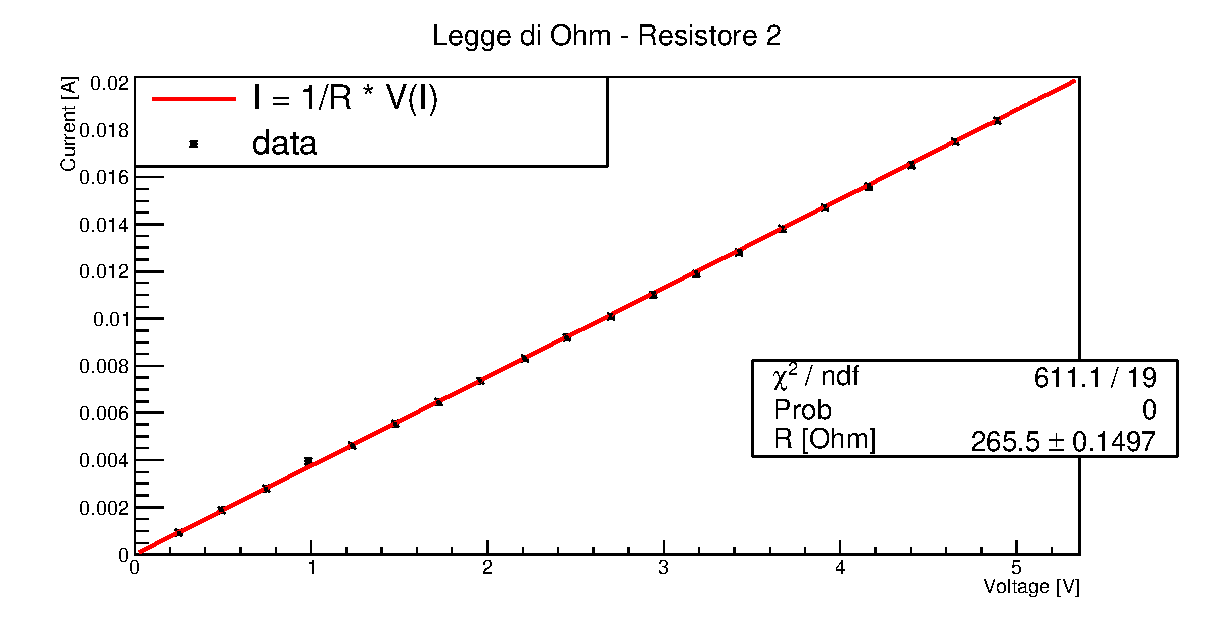
\includegraphics[scale=.8]{Grafici/C1_P1_ohmR2.eps}
    %\caption{Verifica legge di Ohm per resistore R2}
    \label{fig:C1_P1_OhmR2}
    \end{figure}
%
    %   Resistore R2
    \begin{center}
    %\centering
    Valore misurato: $R_2 = 266 \pm 1  \Omega$  \\
    Valore ottenuto dal fit: $ R_2 = 265.5 \pm 0.1 \Omega$ \\
    \end{center}
%
    In questo caso il chi quadro ridotto è molto alto. I dati sono molto scatterati rispetto alla linea, rispetto al loro errore. Siccome il risultato finale è accurato, il problema è probabilmente dovuto ad una sottovalutazione dell'errore associato alle misure.
%
\subsubsection{Resistenze composite}
    Errori considerati come ultima cifra decimale dello strumento di misura.\\
%
    Dati:\\
       $ R_1 = 148 \pm 1 k\Omega $\\ 
       $ R_2 = 149 \pm 1 k\Omega $\\ 
       $ R_3 = 100 \pm 1 k\Omega $\\ 
%     
%
    %Req serie
    \begin{table}[H]
\caption{Misure sperimentali con resistenze in serie}
\begin{tabular}{|c|c|c|c|c|}
\hline
    Combinazione & Tensione V (k$\Omega$) & Corrente I (mA) & Req (k$\Omega$) & Req teorica (k$\Omega$) \\ \hline
     & $\pm$ 0.001 &  $\pm$ 0.001 & $\pm$ 1 & \\ 
     \hline
    R1+R2   & 5.003 & 0.017 & 294 & 297 \\ 
            & 7.500 & 0.026 & 288 & 297 \\
            & 10.02 & 0.035 & 286 & 297 \\
    R1+R3   & 5.009 & 0.021 & 239 & 248 \\
            & 7.500 & 0.031 & 242 & 248 \\
            & 10.01 & 0.041 & 243 & 248 \\
    \hline
\end{tabular}
\label{}
\end{table}
%  
    %Req parallelo
    \begin{table}[H]
\caption{Misure sperimentali con resistenze in Parallelo}
\begin{tabular}{|c|c|c|c|c|}
\hline
    Combinazione & Tensione V (k$\Omega$) & Corrente I (mA) & Req (k$\Omega$) & Req teorica (k$\Omega$) \\ \hline
     & $\pm$ 0.001 &  $\pm$ 0.001 & $\pm$ 0.1 & \\ 
    \hline
    R1+R2   & 5.007 & 0.068 & 73.6 & 74.2 \\
            & 7.500 & 0.102 & 73.5 & 74.2 \\ 
            & 10.01 & 0.136 & 73.6 & 74.2 \\  \hline
    R1+R3   & 5.008 & 0.084 & 59.6 & 59.7 \\ 
            & 7.510 & 0.126 & 59.6 & 59.7 \\ 
            & 10.00 & 0.168 & 59.5 & 59.7 \\ \hline
\end{tabular}
\label{}
\end{table}
    
    Riassunto risultati:
    %risultati resistenza equivalente
    \begin{table}[H]
    \centering
    \caption{Risultati di Resistenza equivalente ottenuti}
    \begin{tabular}{|c|c|c|c|}
        \hline
        SERIE & Teorica (k$\Omega$) & Misurata (k$\Omega$) & Discrepanza \% \\ \hline
        R1+R2 & 297 & 290 $\pm$ 1 & 2\% \\ 
        R1+R3 & 248 & 241 $\pm$ 1 & 3\% \\ 
        \hline
        PARALLELO & Teorica (k$\Omega$) & M (k$\Omega$) & Discrepanza \% \\ \hline
        R1+R2 & 74 & 74 $\pm$ 1 & 1\% \\ 
        R1+R3 & 60 & 60 $\pm$ 1 & 1\% \\ \hline
    \end{tabular}
    \label{}
\end{table}
 
